% !TeX root = ../main.tex
% !TeX encoding = UTF-8

\chapter{Análise de Resultados}

\label{cap:analise_resultados}

\section{Delimitação dos resultados apresentados}

Este capítulo apresenta os resultados da montagem e da execução do ambiente experimental destinado à análise de vulnerabilidades em redes IEEE 802.11 com dispositivos IoT. A apresentação inicia-se pela validação da estação de captura, pela observação funcional de referência de uma câmera IP e por um ensaio piloto de desautenticação contra essa câmera, e segue para o conjunto completo de dispositivos --- câmera IP, lâmpada inteligente, tomada inteligente e \textit{smartphone} de referência ---, nos cenários WPA2 e modo misto WPA2/WPA3. As evidências utilizadas são as saídas de comandos, as capturas de tela, os arquivos de captura de tráfego no formato PCAPNG e os \textit{logs} de \textit{ping} sincronizados, todos analisados com o Wireshark e com a ferramenta de linha de comando \textit{tshark}.



O escopo executado contempla a maior parte do planejamento descrito na metodologia: no cenário WPA2 foram realizadas três repetições independentes por dispositivo para a tomada, a lâmpada e o \textit{smartphone}, com medição dos tempos de indisponibilidade por \textit{ping}; e o cenário com WPA3 habilitado foi incluído na forma de modo misto (WPA2/WPA3). A câmera é um caso à parte: no cenário WPA2, teve duas execuções válidas com \textit{ping} (\texttt{CAM\_WPA2\_R03} e \texttt{CAM\_WPA2\_R04}), além do ensaio piloto, sem \textit{ping}; o arquivo \texttt{CAM\_WPA2\_R02}, apesar do nome, foi gravado com o ponto de acesso em modo misto e é tratado como ensaio desse cenário. Mantêm-se como delimitações esse número reduzido de repetições da câmera (cujo equipamento exige reinício manual a cada teste), o número reduzido de repetições no cenário misto (uma execução para a tomada e para a lâmpada, duas para a câmera e para o \textit{smartphone}) e a impossibilidade de testar os dispositivos IoT em WPA3 puro, uma vez que câmera e tomada não suportam esse protocolo.



Todos os indicadores quantitativos apresentados neste capítulo são derivados diretamente dos arquivos de captura e dos \textit{logs} de \textit{ping}, e não de transcrição manual de imagens: as contagens de quadros, o número de quadros de desautenticação, a duração das capturas, as janelas e taxas de emissão do ataque e a segurança efetivamente negociada por cada dispositivo foram extraídos dos arquivos de captura com o \textit{tshark}, enquanto os tempos sem resposta e as demais métricas de conectividade foram calculados a partir dos \textit{logs} de \textit{ping}. Quanto às ferramentas, a captura do ensaio piloto foi feita com o Wireshark (motor \textit{dumpcap}) e a dos ensaios do conjunto completo com o \textit{tcpdump}, ambos operando o adaptador em modo monitor na Kali Linux; a análise de todas as capturas foi feita com o Wireshark e o \textit{tshark}. O ensaio piloto da câmera, descrito nas seções iniciais, é mantido por documentar a integração inicial do ambiente; os resultados do conjunto completo de dispositivos e a comparação entre os cenários com e sem PMF são apresentados na Seção~\ref{subsec:consolidacao_tabelas}.



\section{Procedimentos de teste}

Esta seção descreve como o ambiente foi efetivamente exercitado e quais instrumentos foram empregados. Por se tratar de um estudo de segurança de redes, e não de um sistema de informação com interface própria, os procedimentos de teste correspondem à verificação funcional da instrumentação, à integração dos componentes do ambiente e a um ensaio direcionado de desautenticação, e não a baterias de testes de software convencionais.

\subsection{Tipos de testes aplicados}

Nesta etapa foram aplicados três tipos de verificação. O primeiro corresponde a um \textbf{teste de validação da estação de captura}, destinado a confirmar que o adaptador em modo monitor registrava quadros IEEE~802.11 no canal da rede de teste. O segundo é um \textbf{teste funcional de referência}, no qual a câmera foi observada em operação normal, sem intervenção da plataforma de baixo custo. O terceiro é um \textbf{ensaio direcionado} ao endereço da câmera, durante o qual foram inspecionados os quadros classificados como \textit{Deauthentication}.

O procedimento foi organizado em uma condição de referência, sem intervenção do LILYGO, e em um ensaio direcionado ao endereço da câmera selecionada. Na referência, o pesquisador relatou funcionamento normal da imagem ao vivo, enquanto a captura apresentou quadros IEEE 802.11 associados ao ponto de acesso e à câmera. No ensaio, foram identificados registros classificados como \textit{Deauthentication}. As durações do ensaio piloto relatadas nesta seção derivam dos tempos relativos da própria captura; os tempos de indisponibilidade por \textit{ping} só foram medidos no conjunto completo de dispositivos (Seção~\ref{subsec:consolidacao_tabelas}).

No ensaio piloto descrito nesta seção não foram aplicados testes sistemáticos de desempenho (tempo de resposta e carga), as três execuções independentes por cenário nem a comparação entre as configurações WPA2 e WPA3. Esses procedimentos foram realizados posteriormente, para o conjunto completo de dispositivos, e são apresentados na Seção~\ref{subsec:consolidacao_tabelas}.

\subsection{Ferramentas e dispositivos utilizados}

A bancada efetivamente utilizada neste ensaio corresponde à descrita na metodologia: o roteador TP-Link EX1500 como ponto de acesso; o LILYGO T-Embed CC1101 Plus (\textit{firmware} Bruce 1.16.1) como plataforma de teste; uma câmera Xiaomi identificada comercialmente como Mi 360 PTZ 2K; um \textit{notebook} com Kali Linux executado em máquina virtual VirtualBox; um adaptador USB Qualcomm Atheros AR9271; e o Wireshark 4.6.6. O ambiente observado utilizou a rede TCC\_LAB em 2,4 GHz, canal 6, com largura de 20 MHz. O protocolo de segurança foi documentado no painel administrativo do roteador, apresentado na Figura~\ref{fig:painel_roteador_wpa2}, que registra a rede TCC\_LAB configurada com segurança WPA2-PSK[AES], isto é, WPA2 com criptografia AES/CCMP. A opção de \textit{Protected Management Frames} (PMF) não aparece habilitada para esse modo nesse \textit{firmware}. Ressalta-se que o painel registra apenas a configuração do ponto de acesso, e não a segurança efetivamente negociada por cada estação; esta é verificada no elemento RSN dos quadros de associação, cujas evidências constam do Apêndice~\ref{sec:evidencias-rsn}. Nas capturas deste cenário, os \textit{beacons} do ponto de acesso anunciam somente o AKM~2 (PSK) e o bit MFPC~=~0, o que confirma, do lado do ponto de acesso, que o PMF não era oferecido; esse estado é coerente com o fato de o ataque de desautenticação ter sido efetivo, uma vez que o PMF, quando ativo, protege justamente os quadros de gerenciamento contra falsificação. Como este ensaio contempla apenas o cenário WPA2, ele não é classificado aqui como comparação entre configurações de segurança, comparação apresentada na Seção~\ref{subsec:consolidacao_tabelas}.

\begin{figure}[htb]
\centering
\caption{Configuração de segurança da rede de teste no painel do roteador}
\label{fig:painel_roteador_wpa2}
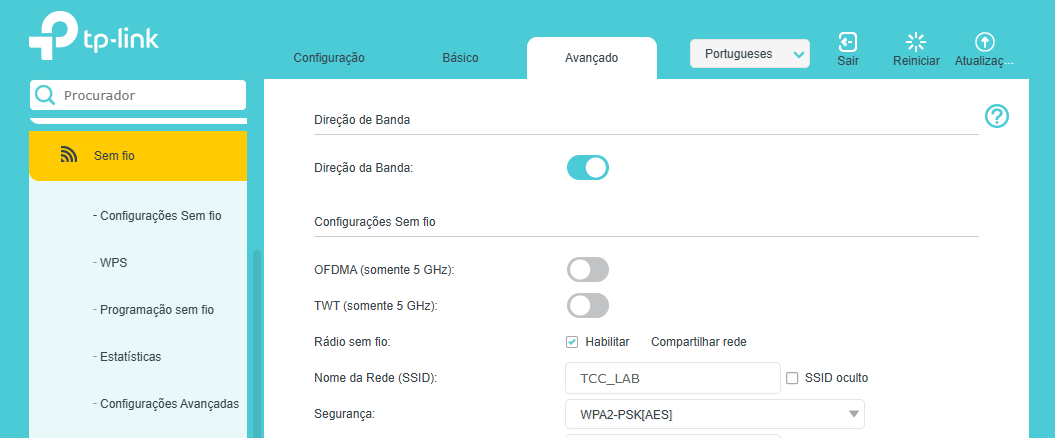
\includegraphics[width=0.9\textwidth]{painel_roteador_wpa2.png}
\legend{Fonte: captura do pesquisador no painel administrativo do TP-Link EX1500 (2026).}
\end{figure}



O Quadro~\ref{quad:config-documentada} reúne os componentes efetivamente utilizados na bancada do ensaio piloto, com seus modelos, versões de \textit{software}/\textit{firmware} e parâmetros de rádio, servindo de referência para a interpretação das evidências apresentadas nas seções seguintes.

\begin{quadro}[htbp]
\centering
\caption{Configuração efetivamente documentada}
\label{quad:config-documentada}
\small
\begin{tabular}{|>{\raggedright\arraybackslash}p{0.45\textwidth}|>{\raggedright\arraybackslash}p{0.45\textwidth}|}
\hline
\textbf{Componente} & \textbf{Registro} \\ \hline
Ponto de acesso & TP-Link EX1500; \textit{firmware} informado 1.13.0 \\ \hline
Plataforma de teste & LILYGO T-Embed CC1101 Plus; Bruce 1.16.1 \\ \hline
Câmera & Xiaomi, nome de rede chuangmi\_camera\_029a02; código de modelo PTZ 2K; \textit{firmware} 4.3.4\_0425 (Seção~\ref{sec:inventario}) \\ \hline
Estação de captura & Kali Linux em VirtualBox; Wireshark 4.6.6 \\ \hline
Adaptador & Qualcomm Atheros AR9271; USB 0cf3:9271; \textit{driver} ath9k\_htc \\ \hline
Condição de rádio & 2,4 GHz; canal 6; 2437 MHz; largura de 20 MHz \\ \hline
Segurança e PMF (configurados) & WPA2-PSK[AES] (AES/CCMP); PMF não habilitado no painel (Figura~\ref{fig:painel_roteador_wpa2}); \textit{beacon}: AKM~2, MFPC~=~0 (Apêndice~\ref{sec:evidencias-rsn}) \\ \hline
Acesso externo & Internet disponibilizada durante a preparação \\ \hline
\end{tabular}
\legend{Fonte: elaborado pelo autor a partir dos registros do ensaio (2026).}
\end{quadro}

\section{Métricas coletadas}

\subsection{Indicadores avaliados}

Os indicadores previstos para o estudo compreendem o funcionamento da câmera na condição de referência, a presença de quadros de desautenticação, o tempo de indisponibilidade funcional, o tempo de recuperação da associação, a ocorrência de recuperação automática, o total de quadros no ensaio, a comparação entre WPA2 e WPA3 e a realização de três repetições por cenário. A situação de cada indicador no ensaio piloto é consolidada ao final desta seção, distinguindo o que foi documentado do que não foi mensurado nesse ensaio; os valores medidos para todos os dispositivos são apresentados na Seção~\ref{subsec:consolidacao_tabelas}.

\subsection{Dicionário de métricas}
\label{subsec:dicionario_metricas}

Antes da apresentação dos resultados, esta subseção define cada métrica utilizada no capítulo e nas Tabelas~\ref{tab:registro-execucoes} e~\ref{tab:registro-metricas}. As definições separam grandezas que, embora relacionadas, não são equivalentes: segundos sem resposta, porcentagem de pacotes perdidos e porcentagem do tempo de observação medem coisas diferentes e não devem ser comparados entre si. Do mesmo modo, a perda de respostas a \textit{ping} não se confunde com a perda de associação, e a recuperação da rede não se confunde com a recuperação da função do dispositivo.

\begin{description}
    \item[Perda de pacotes ICMP (\%):] razão entre as requisições \textit{Echo Request} do \textit{Internet Control Message Protocol} (ICMP) sem resposta válida e o total de requisições enviadas ao dispositivo, multiplicada por 100. O \textit{ping} é executado a partir da estação de captura com o comando \texttt{ping -D -i 0.5}, isto é, com marcas de tempo absolutas e intervalo nominal de 0,5~s entre requisições; não foi definido tempo limite explícito por requisição, pois a opção \texttt{-W} não foi utilizada e, portanto, vigorou o comportamento padrão do \textit{iputils}. O total de requisições e as perdas são obtidos pela contagem dos números de sequência (\texttt{icmp\_seq}): uma sequência é considerada recebida quando há ao menos uma resposta válida com aquele número. As respostas duplicadas (\textit{DUP!}), que no \textit{log} vêm acompanhadas do aviso \textit{wrong data byte} e de tempo \texttt{0.000~ms}, são descartadas por corresponderem a eco de conteúdo corrompido, e não a uma nova resposta válida. A regra vale também para a primeira ocorrência desse eco, que o \textit{ping} não marca como duplicada, mas que traz o mesmo aviso e o mesmo tempo de \texttt{0.000~ms}. A porcentagem só tem sentido junto da janela sobre a qual foi calculada, que deve ser sempre informada.
    \item[Tempo acumulado sem resposta (s):] soma, dentro da janela observada, de todos os intervalos entre respostas válidas consecutivas que excedem o limiar de 2~s. Intervalos menores que o limiar são tratados como variação normal e não entram na soma. É a métrica apresentada como indisponibilidade nas tabelas deste capítulo.
    \item[Fração do tempo sem resposta (\%):] tempo acumulado sem resposta dividido pela duração do \textit{log} de \textit{ping} correspondente, multiplicado por 100. Não equivale à perda de pacotes ICMP nem à fração da janela de ataque, pois o \textit{log} de \textit{ping} pode começar antes e terminar depois do ataque.
    \item[Maior queda contínua (s):] o maior intervalo isolado entre duas respostas válidas consecutivas na janela observada. Distingue-se do tempo acumulado: um dispositivo com muitas quedas curtas pode ter tempo acumulado alto e maior queda contínua baixa, enquanto outro, com uma única queda longa, tem os dois valores iguais.
    \item[Recuperação de rede:] retorno das respostas válidas ao \textit{ping} de forma sustentada após a última queda. Pode ser \textit{automática}, quando ocorre sem intervenção, ou \textit{manual}, quando depende de ação do pesquisador.
    \item[Recuperação da função:] retorno do serviço que o usuário percebe, que é distinto da rede: a imagem ao vivo da câmera no aplicativo, a resposta da tomada a um comando de liga/desliga e a resposta da lâmpada a um comando no aplicativo. Um dispositivo pode voltar a responder a \textit{ping} sem que a função tenha sido restabelecida.
    \item[Perda de associação:] saída do dispositivo do estado associado ao ponto de acesso, confirmada por evidência de enlace, como a ausência de tráfego de dados do dispositivo seguida de quadros de autenticação/associação (reassociação), ou pela remoção do cliente na lista do roteador. \textbf{\textit{Ping} perdido não prova desassociação}, pois a ausência de resposta pode decorrer de congestionamento do canal, de perda de quadros ou de economia de energia do dispositivo.
    \item[Quadros de desautenticação:] número de quadros \textit{Deauthentication} (subtipo 0x0C) na captura, contados com filtro explícito e sempre acompanhados do recorte usado: (i) direcionados ao dispositivo, isto é, com o endereço do dispositivo como origem ou destino; (ii) em difusão (\textit{broadcast}); e (iii) dentro da janela de ataque. O total bruto do arquivo pode incluir quadros de outros clientes e não é usado como medida de intensidade do ataque contra um alvo.
\end{description}

Dois casos especiais seguem regras próprias. Quando o dispositivo não se recupera até o fim da janela observada, o tempo é registrado como limite inferior, na forma ``pelo menos $X$~s, recuperação espontânea não observada'', e não como duração da indisponibilidade. Quando a recuperação exige reinício manual do equipamento, a execução é sinalizada à parte e seu valor não entra no cálculo das médias com as execuções de recuperação espontânea, uma vez que o tempo até o reinício depende da decisão do pesquisador, e não do comportamento do dispositivo. Pela mesma razão, quando algum valor de uma combinação de dispositivo e cenário é limite inferior, a média dessa combinação não é calculada e os valores individuais são apresentados. Na Figura~\ref{fig:comparacao_pmf}, nessas combinações, a barra mostra a média das frações tratada apenas como limite inferior ($\geq$), e os pontos sobre a barra indicam os valores de cada execução.

As métricas de conectividade foram calculadas pelo \textit{script} \texttt{src/analisa\_ping.py}, que lê os \textit{logs} de \textit{ping}, aplica as regras de validade acima e obtém o instante do último quadro de cada captura para identificar as quedas que se estendem até o seu encerramento. Uma versão anterior do cálculo não descartava a primeira ocorrência do eco corrompido; como ela aparece no meio ou no fim de um intervalo sem resposta, essa versão dividia quedas contínuas em duas e, quando o eco era a última linha com resposta, encerrava a queda antes do fim da captura. Os valores apresentados neste capítulo já corrigem esse ponto.

\subsection{Métodos de coleta}

A identificação dos equipamentos e da rede foi obtida pela combinação da lista de clientes do roteador com os campos de endereço dos quadros capturados. Para a apresentação dos resultados, a câmera recebe o identificador CAM-01 e o ponto de acesso AP-01. Os endereços completos permanecem desnecessários à interpretação pública do experimento. O método separa a identificação lógica nos quadros da atribuição física do emissor.



Em uma consulta pontual, o painel do roteador indicou taxa de 72 Mbps e RSSI (\textit{Received Signal Strength Indicator}, indicador de intensidade do sinal recebido) de -39 dBm. Essas leituras caracterizam somente o instante observado e o contexto da interface administrativa: não são médias de sinal nem medições de vazão da aplicação. A análise também não equipara essa leitura à intensidade recebida pelo adaptador de captura.



Os tempos numéricos apresentados neste capítulo correspondem ao tempo relativo de cada captura, medido a partir do seu início (coluna \textit{Time} do Wireshark). São marcas relativas internas ao arquivo, e não horários de relógio; o tempo de recuperação funcional do vídeo, em particular, não é derivado desses valores, pois exigiria registro sincronizado por \textit{ping}. As contagens e taxas de quadros, por sua vez, foram calculadas sobre a totalidade dos quadros de cada arquivo, e não sobre amostras selecionadas.



O tempo de indisponibilidade funcional é calculado entre a primeira perda observável da função e seu restabelecimento, conforme critério previamente definido. No ensaio piloto, por não haver registro de \textit{ping} sincronizado, esse tempo não foi medido diretamente, tendo sido estimado apenas pela interrupção do fluxo de dados da câmera; a mensuração por \textit{ping}, bem como as médias entre repetições e a comparação entre dispositivos e cenários, é apresentada mais adiante, para o conjunto completo de dispositivos, na Seção~\ref{subsec:consolidacao_tabelas}.

O Quadro~\ref{quad:situacao-metricas-ref} resume a situação de cada indicador especificamente no ensaio piloto, distinguindo o que foi documentado do que não foi mensurado nesse ensaio.



\begin{quadro}[htbp]
\centering
\caption{Situação das métricas no ensaio piloto}
\label{quad:situacao-metricas-ref}
\small
\begin{tabular}{|>{\raggedright\arraybackslash}p{0.45\textwidth}|>{\raggedright\arraybackslash}p{0.45\textwidth}|}
\hline
\textbf{Indicador} & \textbf{Situação} \\ \hline
Funcionamento na referência & Normal; câmera transmitindo $\sim$172 quadros de dados/s (8.901 em 51,7~s) \\ \hline
Quadros de desautenticação & 281 quadros no ensaio piloto; \textit{reason code}~7 em 269 (95,7\%) \\ \hline
Indisponibilidade funcional (s) & Fluxo de dados cessou em 75,06~s e não retornou até o fim da captura: pelo menos aproximadamente 68~s ($\approx$67,9~s) sem dados, recuperação espontânea não observada; recuperação do vídeo não cronometrada (reinício manual, fora desse intervalo) \\ \hline
Recuperação da associação (s) & Não mensurada; nenhuma reassociação na captura (0 quadros de \textit{authentication}/\textit{association}) \\ \hline
Recuperação automática & Não observada neste ensaio; vídeo restabelecido por reinício manual \\ \hline
Total de quadros no ensaio & 46.093 quadros em 143,0~s de captura \\ \hline
Comparação WPA2/WPA3 & Não realizada neste ensaio piloto (ensaio em WPA2) \\ \hline
Três repetições por cenário & Não aplicável a este ensaio piloto (execução única) \\ \hline
\end{tabular}
\legend{Fonte: elaborado pelo autor a partir dos registros do ensaio (2026).}
\end{quadro}

\section{Resultados obtidos}

\subsection{Integração dos componentes do ambiente}

Na preparação da estação de captura, a primeira execução de iw dev não apresentou interfaces sem fio. Após o encaminhamento do adaptador USB à máquina virtual, lsusb identificou o dispositivo 0cf3:9271 e iw dev apresentou a interface wlan0. Em seguida, o modo monitor foi ativado, sendo posteriormente confirmada a interface wlan0mon no canal 6, frequência central de 2437 MHz e largura de 20 MHz. Esses registros evidenciam a preparação do instrumento de observação; não representam uma falha do dispositivo IoT.



A câmera foi conectada à rede de laboratório após a disponibilização de internet ao roteador. A dependência observada durante a preparação motivou a manutenção do acesso à internet na condição de referência. Não foi realizado um experimento separado para determinar o funcionamento da câmera ou do aplicativo sem serviços externos. Assim, não se atribui automaticamente todo evento de aplicação à camada de enlace. A integração entre adaptador, máquina virtual, modo monitor e associação da câmera constitui a base sobre a qual os demais resultados foram observados.

\subsection{Testes funcionais}
\label{subsec:testes_funcionais}

A validação da captura, registrada no arquivo \texttt{PREP\_\-01\_\-valida\-cao\_\-captura.\-pcapng}, contém 973 quadros ao longo de 29,2~s, sem nenhum quadro de desautenticação. Nela aparecem quadros Beacon anunciando a rede TCC\_LAB e registros QoS Data, Block Ack, Request-to-send e Clear-to-send envolvendo os endereços identificados na bancada. Esses elementos mostram que a estação de monitoramento registrou classes distintas de quadros IEEE 802.11 no ambiente. A inspeção não autoriza afirmar que todo o tráfego transmitido foi capturado ou que toda a captura se restringe aos dispositivos do laboratório.



Na observação funcional de referência, registrada no arquivo \texttt{D01\_CONTROLE\_R01.pcapng}, o pesquisador informou que a câmera funcionou normalmente. A captura correspondente contém 19.468 quadros ao longo de 51,7~s, sem nenhum quadro de desautenticação, e evidencia um fluxo contínuo de dados da câmera, com 8.901 quadros de dados associados ao seu endereço, o que corresponde a uma média aproximada de 172 quadros de dados por segundo. Essa leitura caracteriza a condição de referência de forma quantitativa; ainda assim, não equivale a uma medição contínua de disponibilidade ou de latência da aplicação de vídeo.



Quanto ao resultado funcional após a intervenção, o pesquisador relatou que, durante o ensaio direcionado ao endereço da câmera, a imagem ao vivo congelou e a transmissão conduzida pela plataforma de teste foi encerrada. Após aproximadamente três minutos sem retorno do vídeo, a câmera foi reiniciada manualmente e a imagem voltou a ser exibida normalmente. Esse relato descreve a percepção funcional do pesquisador; o intervalo de cerca de três minutos é uma estimativa relatada, e não um tempo de recuperação aferido por \textit{ping}, e o restabelecimento ocorreu por reinício manual do equipamento, não por recuperação espontânea.

A análise do arquivo \texttt{PILOTO\_CAM\_C1\_01.pcapng}, entretanto, fornece uma evidência objetiva e sincronizada do início da interrupção. Durante os primeiros 75~s da captura, a câmera manteve um fluxo contínuo de quadros de dados, em média próximo de uma centena de quadros por segundo. O último quadro de dados da câmera foi registrado em $t = 75{,}064$~s, praticamente coincidente com o início da rajada de quadros de desautenticação, observada a partir de $t = 75{,}007$~s. A partir desse instante, e até o encerramento da captura em 143,0~s, não foi registrado nenhum quadro de dados originado pela câmera, o que caracteriza um intervalo de pelo menos aproximadamente 68~s ($\approx$67,9~s, de 75,06~s a 143,0~s) de ausência completa de tráfego de dados do dispositivo dentro da janela observada. Como a rajada de desautenticação durou cerca de 17,6~s (de 75,0~s a 92,6~s) e a câmera permaneceu sem transmitir dados por um período muito superior ao da própria rajada, observa-se que um estímulo breve foi suficiente para provocar uma interrupção prolongada, que só foi revertida por reinício manual.



A correlação temporal entre a rajada de quadros de desautenticação e a interrupção do fluxo de dados da câmera, observada na mesma captura, reforça a interpretação de que o procedimento de desautenticação esteve associado à perda da função. Ainda assim, dois pontos preservam a cautela da análise: trata-se de um único ensaio piloto, não de uma série de repetições que permita afirmar reprodutibilidade; e a identificação lógica dos quadros não comprova que os equipamentos legítimos os originaram fisicamente, pois os endereços de origem podem ser falsificados pela plataforma de teste. Dessa forma, embora a coincidência temporal seja consistente e aponte fortemente para o efeito esperado do ataque, a confirmação definitiva da relação de causa e efeito depende da repetição do ensaio e do registro sincronizado por \textit{ping} do tempo de recuperação funcional. A repetição com registro por \textit{ping} foi realizada posteriormente e é apresentada na Seção~\ref{subsec:consolidacao_tabelas}; o tempo de recuperação funcional, porém, não foi medido.



A Figura~\ref{fig:evidencia_desautenticacao} apresenta, a título de ilustração qualitativa da ferramenta, um recorte da interface do Wireshark com sucessivos quadros rotulados Deauthentication, registrado em um ensaio inicial anterior ao arquivo consolidado nesta análise --- razão pela qual seus números de quadro e instantes diferem dos apresentados nas Tabelas~\ref{tab:metricas-piloto} e~\ref{tab:seis-registros}, derivadas do arquivo \texttt{PILOTO\_CAM\_C1\_01.pcapng}. Os campos exibidos indicam sentidos lógicos tanto de CAM-01 para AP-01 quanto de AP-01 para CAM-01. Essa apresentação não comprova que os equipamentos legítimos originaram fisicamente os quadros, porque a interpretação da origem real requer evidências complementares e correlação com o procedimento de teste.



A composição quantitativa do ensaio piloto foi obtida diretamente do arquivo \texttt{PILOTO\_CAM\_C1\_01.pcapng} e está sintetizada na Tabela~\ref{tab:metricas-piloto}. A captura contém 46.093 quadros ao longo de 143,0~s, dos quais 281 são quadros de desautenticação. Esses quadros concentram-se em uma única janela, entre 75,0~s e 92,6~s, totalizando cerca de 17,6~s de emissão, a uma taxa média próxima de 16 quadros por segundo. Em 269 dos 281 quadros (95,7\%) o campo \textit{reason code} assume o valor 7 (\textit{Class 3 frame received from nonassociated station}), padrão compatível com um ataque de desautenticação em fluxo contínuo.

Quanto ao sentido lógico, os quadros distribuem-se entre o ponto de acesso e a câmera em ambos os sentidos --- 134 de AP-01 para CAM-01 e 132 de CAM-01 para AP-01 --- além de 15 quadros de AP-01 em difusão (\textit{broadcast}). Todos os quadros de desautenticação possuem 66 bytes no arquivo de captura, tamanho que inclui o cabeçalho Radiotap acrescentado pelo adaptador em modo monitor (36 bytes) e o campo FCS (4 bytes); o quadro IEEE~802.11 propriamente dito tem 30 bytes, sendo 24 de cabeçalho MAC, 2 de \textit{reason code} e 4 de FCS. A Tabela~\ref{tab:seis-registros} apresenta seis quadros representativos extraídos dessa captura, distribuídos ao longo da janela de ataque, e a Figura~\ref{fig:impacto_deauth_camera} relaciona, no eixo temporal, a emissão dos quadros de desautenticação com a interrupção do fluxo de dados da câmera.

\begin{table}[htbp]
\centering
\caption{Métricas do ensaio piloto de desautenticação (câmera, WPA2)}
\label{tab:metricas-piloto}
\small
\begin{tabular}{|>{\raggedright\arraybackslash}p{0.55\textwidth}|>{\raggedright\arraybackslash}p{0.35\textwidth}|}
\hline
\textbf{Métrica} & \textbf{Valor} \\ \hline
Duração da captura & 143,0 s \\ \hline
Total de quadros na captura & 46.093 \\ \hline
Quadros de desautenticação & 281 \\ \hline
Janela de emissão dos deauth & 75,0 s a 92,6 s ($\approx$17,6 s) \\ \hline
Taxa média de deauth & $\approx$16 quadros/s \\ \hline
\textit{Reason code} predominante & 7 --- \textit{Class 3 frame} (269 de 281; 95,7\%) \\ \hline
Tamanho dos quadros deauth & 66 bytes (36 de Radiotap + 30 do quadro 802.11, com FCS) \\ \hline
Último quadro de dados da câmera & 75,06 s \\ \hline
Quadros de dados da câmera após o ataque & 0 (de 93 s até 143 s) \\ \hline
Reassociação observada na captura & Nenhuma (0 quadros de \textit{auth}/\textit{assoc}) \\ \hline
\end{tabular}
\legend{Fonte: elaborado pelo autor a partir do arquivo \texttt{PILOTO\_CAM\_C1\_01.pcapng} (2026).}
\end{table}



\begin{figure}[htbp]\centering

\caption{Recorte de quadros de desautenticação no ensaio inicial}

\label{fig:evidencia_desautenticacao}

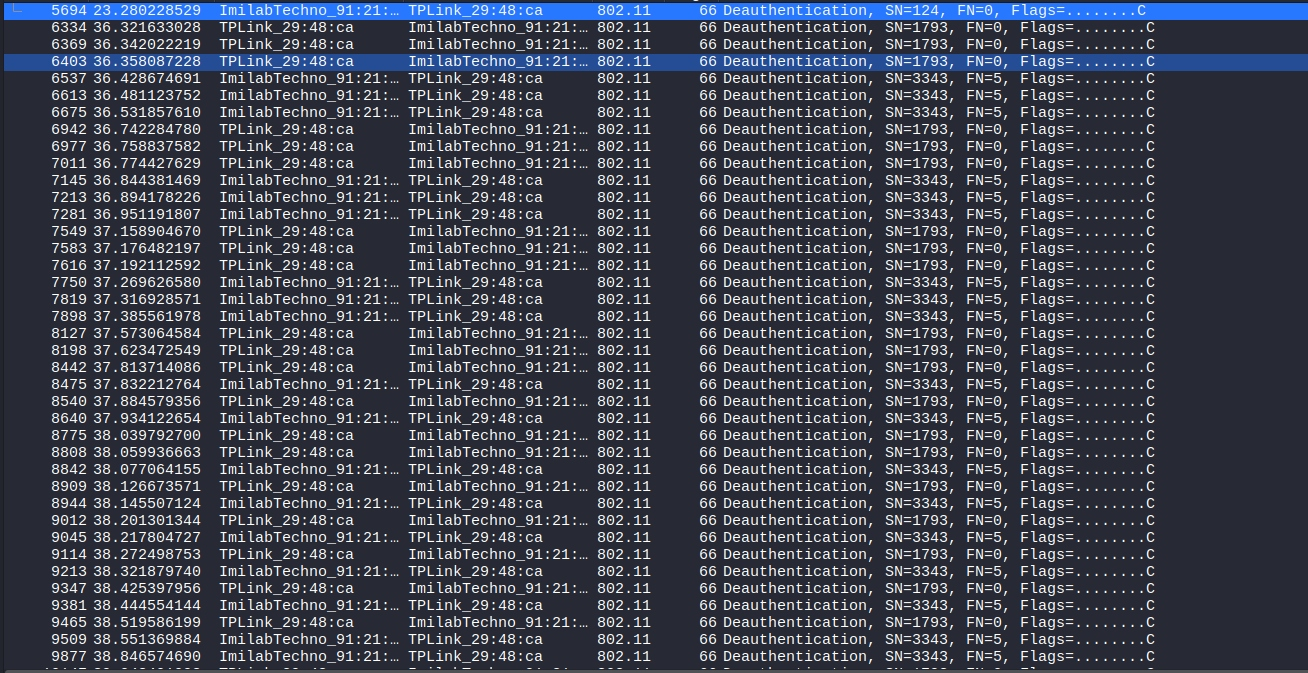
\includegraphics[width=\textwidth]{evidencia_desautenticacao.png}

\legend{Fonte: captura do pesquisador no Wireshark (2026).}

\end{figure}

\begin{table}[htbp]
\centering
\caption{Quadros de desautenticação representativos do ensaio piloto}
\label{tab:seis-registros}
\small
\begin{tabular}{|>{\raggedright\arraybackslash}p{0.16\textwidth}|>{\raggedright\arraybackslash}p{0.26\textwidth}|>{\raggedright\arraybackslash}p{0.32\textwidth}|>{\raggedright\arraybackslash}p{0.12\textwidth}|}
\hline
\textbf{Quadro} & \textbf{Tempo relativo (s)} & \textbf{Sentido lógico} & \textbf{\textit{Reason code}} \\ \hline
19227 & 75,007 & AP-01 $\rightarrow$ CAM-01 & 7 \\ \hline
19494 & 75,163 & CAM-01 $\rightarrow$ AP-01 & 7 \\ \hline
31997 & 83,825 & CAM-01 $\rightarrow$ AP-01 & 7 \\ \hline
32128 & 83,927 & AP-01 $\rightarrow$ CAM-01 & 7 \\ \hline
43822 & 92,127 & CAM-01 $\rightarrow$ AP-01 & 7 \\ \hline
44528 & 92,614 & AP-01 $\rightarrow$ \textit{Broadcast} & 7 \\ \hline
\end{tabular}
\legend{Fonte: elaborado pelo autor a partir do arquivo \texttt{PILOTO\_CAM\_C1\_01.pcapng} (2026).}
\end{table}

\begin{figure}[htbp]\centering

\caption{Impacto do ataque de desautenticação sobre o fluxo de dados da câmera}

\label{fig:impacto_deauth_camera}

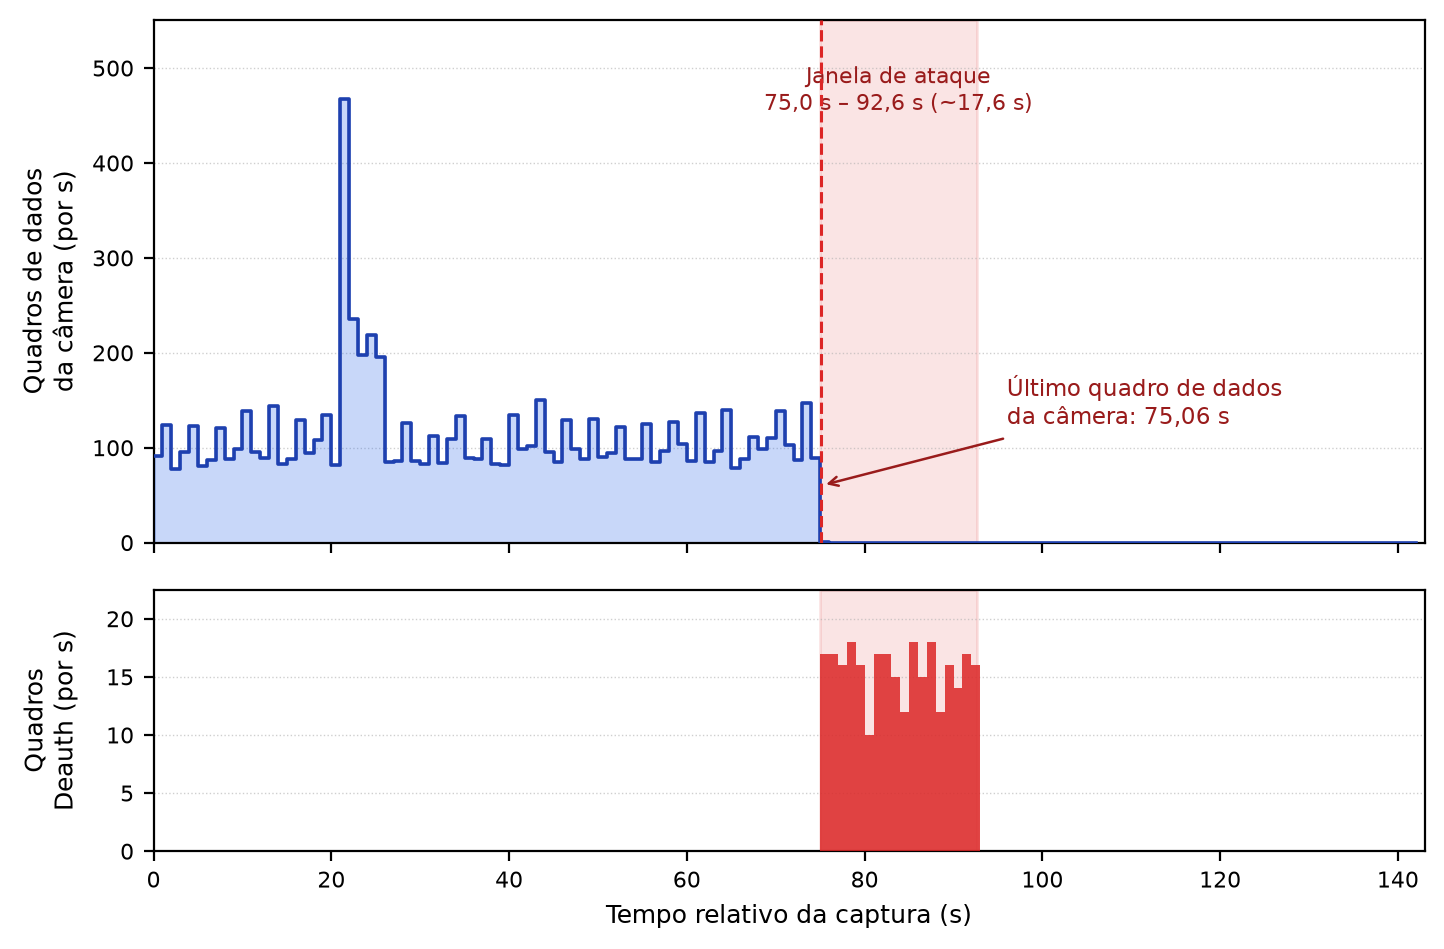
\includegraphics[width=\textwidth]{impacto_deauth_camera.png}

\legend{Fonte: elaborado pelo autor a partir do arquivo \texttt{PILOTO\_CAM\_C1\_01.pcapng} (2026). O painel superior mostra os quadros de dados da câmera por segundo; o inferior, os quadros de desautenticação por segundo. A região sombreada indica a janela de emissão do ataque.}

\end{figure}

\subsection{Desempenho e tempos}

Com a análise dos arquivos de captura, parte dos indicadores de desempenho previstos na metodologia pôde ser efetivamente mensurada nesta etapa, conforme consolidado no Quadro~\ref{quad:situacao-metricas-ref} e na Tabela~\ref{tab:metricas-piloto}. Foram calculados, a partir do arquivo do ensaio piloto, o total de quadros (46.093), o número de quadros de desautenticação (281), a duração da captura (143,0~s), a janela e a taxa de emissão do ataque ($\approx$17,6~s a $\approx$16 quadros/s) e o instante de interrupção do fluxo de dados da câmera (75,06~s), que não voltou a transmitir dados até o fim da captura.

Não foram mensurados, entretanto, o tempo de recuperação funcional do vídeo e o tempo de reassociação do dispositivo no ensaio piloto. O primeiro dependeria de registro sincronizado por \textit{ping} ou por cronômetro, não realizado nesse ensaio; o segundo não pôde ser obtido porque a câmera não se reassociou dentro da janela capturada, tendo sido restabelecida apenas por reinício manual após o encerramento da captura. Esses valores não são estimados por substituição.

\subsection{Segurança negociada por dispositivo}
\label{subsec:consolidacao_resultados}

Após o ensaio piloto com a câmera, o estudo foi estendido ao conjunto completo de dispositivos previsto na metodologia --- câmera IP, lâmpada inteligente, tomada inteligente e \textit{smartphone} de referência ---, em dois cenários de segurança: WPA2 (modo WPA2-PSK[AES]) e um cenário com WPA3 habilitado no roteador em modo misto (WPA2-PSK[AES]+WPA3-Personal), conforme a configuração apresentada na Figura~\ref{fig:painel_roteador_wpa3}. Para cada ensaio foram registrados, de forma sincronizada, o arquivo de captura (gravado pelo \textit{tcpdump} com o adaptador em modo monitor e analisado posteriormente com o \textit{tshark}) e um \textit{log} de \textit{ping} com marcas de tempo (intervalo de 0,5~s), permitindo medir diretamente o tempo de indisponibilidade de cada dispositivo. No cenário WPA2, foram realizadas três repetições independentes para a tomada, a lâmpada e o \textit{smartphone} e duas para a câmera com \textit{ping} (\texttt{CAM\_WPA2\_R03} e \texttt{CAM\_WPA2\_R04}), além do ensaio piloto descrito anteriormente, que não teve \textit{ping}. Uma terceira execução (\texttt{CAM\_WPA2\_R08}) tem linha de base sem ataque, mas o \textit{log} de \textit{ping} apresentou avisos de retrocesso do relógio; por isso, a sua descrição usa os quadros de dados da captura, medida que não foi validada, pois na R03 os dados da câmera não mostram a indisponibilidade observada pelo \textit{ping}. Essa execução é descritiva e não entra nas médias. As execuções \texttt{CAM\_WPA2\_R05} e \texttt{CAM\_WPA2\_R06} foram invalidadas, porque não houve linha de base com respostas normais ao \textit{ping} antes do primeiro quadro de desautenticação direcionado à câmera (Seção~\ref{sec:criterios_validacao}); nenhuma delas entra nas médias. Nas duas execuções da câmera, a função só foi restabelecida após reinício manual; na segunda, o reinício foi feito com a captura em andamento, para registrar o tempo de retorno. No cenário em modo misto, foi realizada uma execução por dispositivo, com duas exceções: a câmera, cujos dois ensaios com \textit{ping} (os arquivos \texttt{CAM\_WPA2\_R02} e \texttt{CAM\_WPA3\_R01}) foram gravados com o ponto de acesso em modo misto; e o \textit{smartphone}, com duas execuções válidas. Nas combinações com uma única execução, cada valor descreve apenas aquela execução e não permite estimar a variação entre repetições. A Tabela~\ref{tab:consolidacao-resultados} consolida os resultados, e a Tabela~\ref{tab:negociacao-seguranca} documenta a segurança negociada por cada dispositivo, obtida do elemento RSN dos quadros de associação nas capturas (Apêndice~\ref{sec:evidencias-rsn}).

Cabe registrar uma restrição de \textit{hardware} relevante para o escopo dos testes. Tanto o microcontrolador LILYGO T-Embed CC1101 Plus, baseado no ESP32-S3 (SoC com dois núcleos Xtensa LX7 e Wi-Fi IEEE~802.11 b/g/n somente em 2,4~GHz, distinto do ESP32 original, de núcleos LX6) \cite{EspressifS3Datasheet}, quanto o adaptador de captura Qualcomm Atheros AR9271 operam exclusivamente na faixa de 2,4~GHz (IEEE 802.11 b/g/n), pois seu \textit{front-end} de rádio não contempla a faixa de 5~GHz. O rádio Wi-Fi do ESP32-S3 é monobanda em 2,4~GHz, de modo que o \textit{firmware} Bruce só consegue injetar quadros de desautenticação nessa faixa; de forma análoga, o AR9271, em modo monitor, só captura tráfego em 2,4~GHz. Por isso, o \textit{smartphone} de referência (Samsung Galaxy S21), inicialmente associado à rede em 5~GHz (canal 157), precisou ser forçado à banda de 2,4~GHz --- desabilitando-se a direção de banda (\textit{band steering}) no roteador --- para ser incluído nos ensaios. Essa restrição é, a um só tempo, uma limitação do estudo e uma observação de segurança: dispositivos que operam exclusivamente em 5~GHz ficam fora do alcance desta plataforma de ataque de baixo custo, baseada em ESP32-S3. A restrição de faixa não se confunde com a segurança negociada: operar em 2,4~GHz não impede o uso de WPA3 ou de PMF, como mostra a própria lâmpada avaliada (Apêndice~\ref{sec:evidencias-rsn}).

Um aspecto determinante para a interpretação dos resultados foi verificado nos quadros de gerenciamento: no cenário em modo misto, cada dispositivo negocia a segurança que suporta, e a configuração exibida no painel do roteador (Figura~\ref{fig:painel_roteador_wpa3}) informa apenas o que o ponto de acesso oferece. Nesse cenário, os \textit{beacons} anunciam os AKM~2 (PSK) e~8 (SAE), com MFPC~=~1 e MFPR~=~0, isto é, PMF oferecido de forma opcional. O campo \textit{Authentication algorithm} do quadro de autenticação não foi tomado como evidência, pois o valor 0 (\textit{Open System}) precede tanto o WPA2-PSK sem PMF quanto o WPA2-PSK com PMF; a evidência adotada é o elemento RSN do \textit{Association Request}, que informa o AKM selecionado e os bits MFPC e MFPR da estação. Por esse critério, a câmera e a tomada selecionaram o AKM~2 (PSK) com MFPC~=~0 e MFPR~=~0, de modo que o PMF não foi negociado, embora oferecido pelo ponto de acesso. A lâmpada, em captura dedicada feita após o seu reinício, realizou a troca SAE (\textit{authentication algorithm}~3) e selecionou o AKM~8 (SAE) com MFPC~=~1 e MFPR~=~1. Para o \textit{smartphone}, que permaneceu associado durante todas as capturas do cenário misto, nenhum quadro de autenticação ou associação foi registrado, e o AKM selecionado não pôde ser observado (AKM não observado); há apenas o indício indireto de que os quadros de gerenciamento do tipo \textit{Action} trocados com o ponto de acesso tinham o bit \textit{Protected} ativo, compatível com PMF negociado, mas incapaz de distinguir SAE de PSK com PMF. Os números dos quadros e os campos de cada evidência constam do Apêndice~\ref{sec:evidencias-rsn}.

\begin{figure}[htb]
\centering
\caption{Configuração da rede em modo misto WPA2/WPA3 no painel do roteador}
\label{fig:painel_roteador_wpa3}
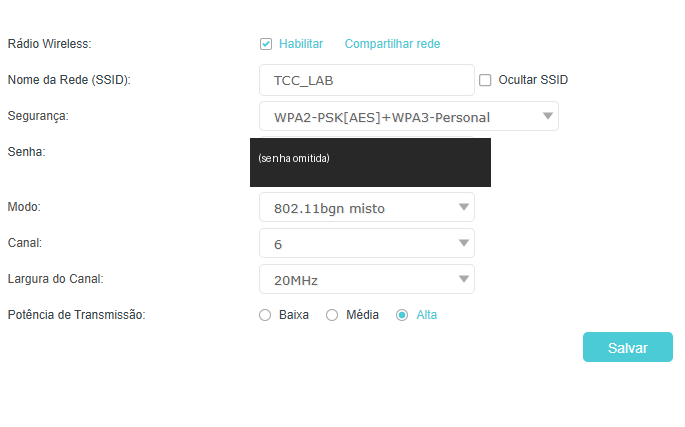
\includegraphics[width=0.82\textwidth]{painel_roteador_wpa3.png}
\legend{Fonte: captura do pesquisador no painel administrativo do TP-Link EX1500 (2026). A senha foi omitida.}
\end{figure}

\begin{table}[htbp]
\centering
\caption[Segurança negociada por dispositivo (modo misto)]{Segurança negociada por cada dispositivo no cenário misto WPA2/WPA3}
\label{tab:negociacao-seguranca}
\marcadoresTabela
\small
\begin{tabular}{|>{\raggedright\arraybackslash}p{0.19\textwidth}|>{\raggedright\arraybackslash}p{0.17\textwidth}|>{\raggedright\arraybackslash}p{0.17\textwidth}|>{\raggedright\arraybackslash}p{0.14\textwidth}|>{\raggedright\arraybackslash}p{0.20\textwidth}|}
\hline
\textbf{Dispositivo} & \textbf{AKM selecionado} & \textbf{MFPC / MFPR (estação)} & \textbf{PMF negociado} & \textbf{Perda de associação observada} \\ \hline
Câmera IP & 2 (PSK) & 0 / 0 & Não & Sim (em 1 de 2 execuções) \\ \hline
Tomada inteligente & 2 (PSK) & 0 / 0 & Não & Sim \\ \hline
Lâmpada inteligente & 8 (SAE)\textsuperscript{a} & 1 / 1 & Sim & Não \\ \hline
\textit{Smartphone} (ref.) & Não observado\textsuperscript{b} & Não observado & Indício indireto\textsuperscript{b} & Não (manteve a associação) \\ \hline
\end{tabular}
\legend{Fonte: elaborado pelo autor a partir do elemento RSN dos quadros de \textit{Association Request} nas capturas (2026); números dos quadros no Apêndice~\ref{sec:evidencias-rsn}. Ponto de acesso no cenário misto: AKM~2 e~8, MFPC~=~1, MFPR~=~0. ``Perda de associação observada'': presença de novas autenticações e associações da estação na captura do ensaio. \textsuperscript{a}Obtido em captura dedicada, após o reinício da lâmpada, e não durante o ensaio de ataque. \textsuperscript{b}Nenhuma associação do \textit{smartphone} foi capturada no cenário misto; quadros de gerenciamento \textit{Action} com o bit \textit{Protected} ativo indicam PMF, sem identificar o AKM. Manter a associação não significa ausência de impacto: o \textit{smartphone} registrou intervalos sem resposta a \textit{ping} (Figura~\ref{fig:comparacao_pmf}).}
\end{table}

A Tabela~\ref{tab:negociacao-seguranca} mostra que a coluna decisiva é a do PMF negociado, e não o rótulo do cenário: câmera e tomada, que não declaram MFPC, operaram sem PMF mesmo com o ponto de acesso oferecendo-o; a tomada e a câmera, em uma das duas execuções (\texttt{CAM\_WPA3\_R01}), apresentaram novas autenticações e associações durante o ataque; a lâmpada, com PMF obrigatório, e o \textit{smartphone}, com indício indireto de PMF, mantiveram a associação. Para o \textit{smartphone}, a última coluna registra apenas a manutenção da associação, e não proteção completa, pois houve intervalos sem resposta a \textit{ping}.

\subsection{Consolidação dos resultados por dispositivo e cenário}
\label{subsec:consolidacao_tabelas}

Os resultados consolidados estão divididos em duas tabelas, para que cada linha informe o número de execuções ($n$) que a sustenta. A Tabela~\ref{tab:consolidacao-resultados} reúne os indicadores de conectividade: a quantidade de quadros de desautenticação direcionados ao dispositivo e o tempo acumulado sem resposta a \textit{ping}, conforme definido na Seção~\ref{subsec:dicionario_metricas}. Nas linhas com uma única execução, o número exibido é o valor observado nessa execução, e não uma média; nas linhas com mais de uma execução, são apresentados os valores individuais, a média e a amplitude (diferença entre o maior e o menor valor), exceto quando algum valor é limite inferior ($\geq$), caso em que a média não é calculada. Os valores de cada execução, com a respectiva janela de ataque, constam das Tabelas~\ref{tab:registro-execucoes} e~\ref{tab:registro-metricas}.

\renewcommand{\arraystretch}{1.2}
\begin{table}[htbp]
\centering
\caption{Consolidação dos resultados por dispositivo e cenário: conectividade}
\label{tab:consolidacao-resultados}
\marcadoresTabela
\scriptsize
\setlength{\tabcolsep}{2.5pt}
\begin{tabular}{|>{\raggedright\arraybackslash}p{0.11\textwidth}|>{\raggedright\arraybackslash}p{0.075\textwidth}|>{\raggedright\arraybackslash}p{0.05\textwidth}|>{\raggedright\arraybackslash}p{0.09\textwidth}|>{\raggedright\arraybackslash}p{0.09\textwidth}|>{\raggedright\arraybackslash}p{0.09\textwidth}|>{\raggedright\arraybackslash}p{0.09\textwidth}|>{\raggedright\arraybackslash}p{0.10\textwidth}|>{\raggedright\arraybackslash}p{0.10\textwidth}|}
\hline
\textbf{Dispositivo} & \textbf{Cenário} & \textbf{$n$} & \textbf{Deauth no disp.} & \multicolumn{3}{>{\centering\arraybackslash}p{0.28\textwidth}|}{\textbf{Tempo acumulado sem resposta por execução (s)}} & \textbf{Média ou valor observado (s)} & \textbf{Amplitude (s)} \\ \cline{5-7}
 & & & & \textbf{R01} & \textbf{R02} & \textbf{R03} & & \\ \hline
Câmera IP & WPA2 & 2 & 625,5 (média) & \multicolumn{3}{c|}{R03: $\geq$160,1; R04: 82,4} & não calculada\textsuperscript{d} & --- \\ \hline
Câmera IP & misto\textsuperscript{a} & 2 & 519,5 (média) & $\geq$55,8 & $\geq$56,5 & --- & não calculada\textsuperscript{a} & --- \\ \hline
Tomada & WPA2 & 3 & 467 (média) & $\geq$45,4\textsuperscript{b} & 106,4 & 93,6 & não calculada\textsuperscript{b} & --- \\ \hline
Tomada & misto & 1 & 712 & \multicolumn{3}{c|}{execução única} & 72,5 (observado) & --- \\ \hline
Lâmpada & WPA2 & 3 & 405 (média) & 40,1 & 49,4 & 52,8 & 47,4 (média) & 12,7 \\ \hline
Lâmpada & misto & 1 & 425 & \multicolumn{3}{c|}{execução única} & 0,0 (observado) & --- \\ \hline
\textit{Smartphone} & WPA2 & 3 & 502 (média) & 73,1 & 66,5 & 65,3 & 68,3 (média) & 7,8 \\ \hline
\textit{Smartphone} & misto\textsuperscript{c} & 2 & 578 (média) & 22,8 & inválida & 24,7 & 23,8 (média) & 1,9 \\ \hline
\end{tabular}
\legend{Fonte: elaborado pelo autor a partir dos arquivos de captura e dos \textit{logs} de \textit{ping} (2026). ``Misto'': WPA3 habilitado em modo misto (WPA2-PSK[AES]+WPA3-Personal). ``Deauth no disp.'': quadros de desautenticação com o endereço do dispositivo como origem ou destino (média das execuções, nas linhas com $n>1$). Tempo acumulado sem resposta: soma dos intervalos sem resposta a \textit{ping} acima de 2~s, excluídas as respostas duplicadas (\textit{DUP!}). A câmera em WPA2 teve duas execuções com \textit{ping} (\texttt{CAM\_WPA2\_R03} e \texttt{CAM\_WPA2\_R04}, nota d); o ensaio piloto não teve \textit{ping} (Tabela~\ref{tab:metricas-piloto}). \textsuperscript{a}As duas execuções da câmera em modo misto correspondem aos arquivos \texttt{CAM\_WPA2\_R02} ($\geq$55,8~s, sem reassociação, exigiu reinício manual) e \texttt{CAM\_WPA3\_R01} ($\geq$56,5~s, com reassociações durante o ataque, mas sem resposta válida a \textit{ping} até o fim da captura; reiniciada manualmente após o fim da captura, com retorno não registrado); em ambos o AP anunciava modo misto e a câmera negociou PSK sem PMF (Apêndice~\ref{sec:evidencias-rsn}). Nas duas execuções, a queda vai até o encerramento da captura, de modo que os valores são limites inferiores e a média não é calculada. \textsuperscript{b}A execução \texttt{TOMADA\_WPA2\_R01} foi registrada com intervalo de \textit{ping} de 1~s (as demais, 0,5~s) e com menor número de quadros de desautenticação direcionados à tomada (49, contra 843 e 510); a última resposta válida ocorreu aos 104,8~s do \textit{log}, e o \textit{ping} prosseguiu sem resposta válida até o fim da captura, enquanto a tomada se reassociava repetidamente; por isso o valor é limite inferior e a média não é calculada. \textsuperscript{c}O \textit{smartphone} em modo misto teve a execução \texttt{PHONE\_WPA3\_R02} invalidada por não conter quadros de desautenticação direcionados a ele (Seção~\ref{sec:criterios_validacao}); a média usa as duas execuções válidas (\texttt{R01} e \texttt{R03}). \textsuperscript{d}Câmera em WPA2: \texttt{CAM\_WPA2\_R03} não teve associação da câmera registrada na captura; o último \textit{ping} válido ocorreu aos 94,9~s da captura, e o intervalo sem resposta termina apenas com o encerramento da captura, aos 254,9~s, por isso o valor é um limite inferior ($\geq$160~s). O reinício foi feito depois desse encerramento. \texttt{CAM\_WPA2\_R04} teve oito trocas de autenticação e associação durante o ataque (entre 88,6 e 95,5~s, todas com \textit{status} 0), cada uma seguida de novo quadro de desautenticação, e uma nova associação após o reinício (184,5~s); o tempo sem resposta forma uma única queda contínua de 82,4~s, calculada sobre respostas válidas. Os \textit{logs} de \textit{ping} das duas execuções registram avisos de retrocesso do relógio, após os quais aparecem apenas linhas \texttt{icmp\_seq=0 (DUP!)}, excluídas do cálculo. A média não é calculada porque um dos valores é limite inferior. A execução \texttt{CAM\_WPA2\_R05} foi invalidada (Seção~\ref{sec:criterios_validacao}) e não entra nesta tabela (Tabelas~\ref{tab:registro-execucoes} e~\ref{tab:registro-metricas}, nota i). A execução \texttt{CAM\_WPA2\_R08}, medida pela captura porque o \textit{log} de \textit{ping} não é confiável, também não entra nas médias por \textit{ping} (Tabelas~\ref{tab:registro-execucoes} e~\ref{tab:registro-metricas}, nota j).}
\end{table}

A Tabela~\ref{tab:consolidacao-recuperacao} complementa a anterior com os indicadores de recuperação: a maior queda contínua, a forma de recuperação da rede e da função do dispositivo, a necessidade de intervenção manual e o resultado de cada combinação de dispositivo e cenário, segundo as quatro categorias definidas na metodologia. A separação entre recuperação de rede e recuperação da função é necessária porque o retorno das respostas a \textit{ping} não garante que a imagem da câmera ou o comando da tomada e da lâmpada tenham voltado a funcionar.

\begin{table}[htbp]
\centering
\caption{Consolidação dos resultados por dispositivo e cenário: recuperação}
\label{tab:consolidacao-recuperacao}
\marcadoresTabela
\scriptsize
\setlength{\tabcolsep}{3pt}
\begin{tabular}{|>{\raggedright\arraybackslash}p{0.115\textwidth}|>{\raggedright\arraybackslash}p{0.08\textwidth}|>{\raggedright\arraybackslash}p{0.035\textwidth}|>{\raggedright\arraybackslash}p{0.118\textwidth}|>{\raggedright\arraybackslash}p{0.15\textwidth}|>{\raggedright\arraybackslash}p{0.13\textwidth}|>{\raggedright\arraybackslash}p{0.075\textwidth}|>{\raggedright\arraybackslash}p{0.17\textwidth}|}
\hline
\textbf{Dispositivo} & \textbf{Cenário} & \textbf{$n$} & \textbf{Maior queda contínua (s)} & \textbf{Recuperação de rede} & \textbf{Recuperação da função} & \textbf{Interv. manual} & \textbf{Resultado} \\ \hline
Câmera IP & WPA2 & 2 & $\geq$160 (R03); 82,4 (R04) & não observada até o fim da captura (R03); retorno só após reinício manual (R04) & não mensurada & Sim em 2 de 2 & Desassociação confirmada em R04; não confirmada em R03 (ver Tabela~\ref{tab:consolidacao-resultados}) \\ \hline
Câmera IP & misto & 2 & $\geq$55,8 e $\geq$51,3 & não espontânea (\texttt{CAM\_\allowbreak{}WPA2\_\allowbreak{}R02}) / não observada até o fim da captura (\texttt{CAM\_\allowbreak{}WPA3\_\allowbreak{}R01}) & não mensurada & Sim em 2 de 2\textsuperscript{a} & Desassociação confirmada em \texttt{CAM\_WPA3\_R01}\textsuperscript{a} \\ \hline
Tomada & WPA2 & 3 & $\geq$33,2; 80,7; 48,3 (média não calculada) & automática (intermitente)\textsuperscript{c} & não mensurada & Não & Desassociação confirmada \\ \hline
Tomada & misto & 1 & 63,3 & automática (intermitente) & não mensurada & Não & Desassociação confirmada \\ \hline
Lâmpada & WPA2 & 3 & 47,4 (média) & automática (intermitente) & não mensurada & Não & Desassociação confirmada \\ \hline
Lâmpada & misto & 1 & 0,0 & não afetada & não mensurada & Não & Sem efeito detectado \\ \hline
\textit{Smartphone} & WPA2 & 3 & 65,1 (média) & manual (seleção da rede) & não mensurada & Sim & Desassociação confirmada \\ \hline
\textit{Smartphone} & misto & 2 & 5,5 (média) & não afetada (manteve associação) & não mensurada & Não & Perda de conectividade sem desassociação confirmada\textsuperscript{b} \\ \hline
\end{tabular}
\legend{Fonte: elaborado pelo autor a partir dos arquivos de captura e dos \textit{logs} de \textit{ping} (2026). ``Maior queda contínua'': maior intervalo isolado sem resposta a \textit{ping}; valor médio nas linhas com $n>1$, exceto quando algum valor é limite inferior ($\geq$), caso em que os valores individuais são listados. ``Desassociação confirmada'' foi atribuída quando a captura registra novos quadros de autenticação e de \textit{Association Request} com o endereço do dispositivo durante o ataque; ``recuperação da função'' não foi mensurada por \textit{ping}. \textsuperscript{a}As duas execuções da câmera em modo misto diferiram: em \texttt{CAM\_WPA2\_R02} não houve reassociação na captura (perda de conectividade sem desassociação confirmada; recuperação só por reinício manual), ao passo que em \texttt{CAM\_WPA3\_R01} a câmera reassociou-se várias vezes durante o ataque (desassociação confirmada), mas não voltou a responder a \textit{ping} nem a transmitir quadros de dados até o fim da captura, encerrada 6,8~s após o fim do ataque; a câmera foi reiniciada manualmente após o fim da captura, e o retorno não foi registrado. \textsuperscript{b}O \textit{smartphone} manteve a associação (nenhum quadro de autenticação ou associação dele na captura), mas registrou intervalos sem resposta a \textit{ping}. \textsuperscript{c}Em \texttt{TOMADA\_WPA2\_R01}, a retomada não foi observada até o fim da captura, encerrada logo após o fim do ataque.}
\end{table}
\renewcommand{\arraystretch}{1.0}

A Figura~\ref{fig:comparacao_pmf} sintetiza o achado central do estudo, apresentando, para cada dispositivo e cenário, a fração do tempo sem resposta a \textit{ping} (Seção~\ref{subsec:dicionario_metricas}); a cor indica se o dispositivo negociou ou não o PMF, o hachurado distingue o cenário misto do cenário WPA2 e os pontos sobre cada barra marcam as execuções individuais. Abaixo de cada barra é indicado o número de execuções ($n$); as barras com $n > 1$ mostram a média, e as barras com $n = 1$, o valor observado. As barras marcadas com $\geq$ incluem ao menos uma execução cuja queda durou até o fim da captura; nesses casos, o valor é um limite inferior. Sem PMF, todos os casos apresentaram fração expressiva de tempo sem resposta: no cenário WPA2, de $\approx$43\% (lâmpada) a $\approx$59\% (\textit{smartphone}), com a câmera ($\geq$51\%) e a tomada ($\geq$47\%) representadas por limites inferiores; e no cenário misto, em que câmera e tomada negociaram PSK sem PMF, de $\geq$53\% (câmera, limites inferiores de 56\% e 50\% em duas execuções) a $\approx$71\% (tomada). Com PMF (lâmpada, com PMF obrigatório negociado; \textit{smartphone}, com indício indireto de PMF), a lâmpada não apresentou intervalos sem resposta na janela observada e o \textit{smartphone}, embora tenha mantido a associação, registrou em média $\approx$22\% do tempo sem resposta (14\% e 29\% em duas execuções). Portanto, câmera e tomada permaneceram sem PMF mesmo com o WPA3 habilitado no roteador em modo misto. No cenário WPA2, a câmera aparece na figura com as execuções \texttt{CAM\_WPA2\_R03} ($\geq$63\%, limite inferior) e \texttt{CAM\_WPA2\_R04} ($\approx$38\%); as demais execuções da câmera nesse cenário não entram, pelos motivos indicados nas Tabelas~\ref{tab:consolidacao-resultados} e~\ref{tab:consolidacao-recuperacao}.

\begin{figure}[htb]
\centering
\caption{Tempo sem resposta a \textit{ping} por dispositivo e cenário, com e sem PMF}
\label{fig:comparacao_pmf}
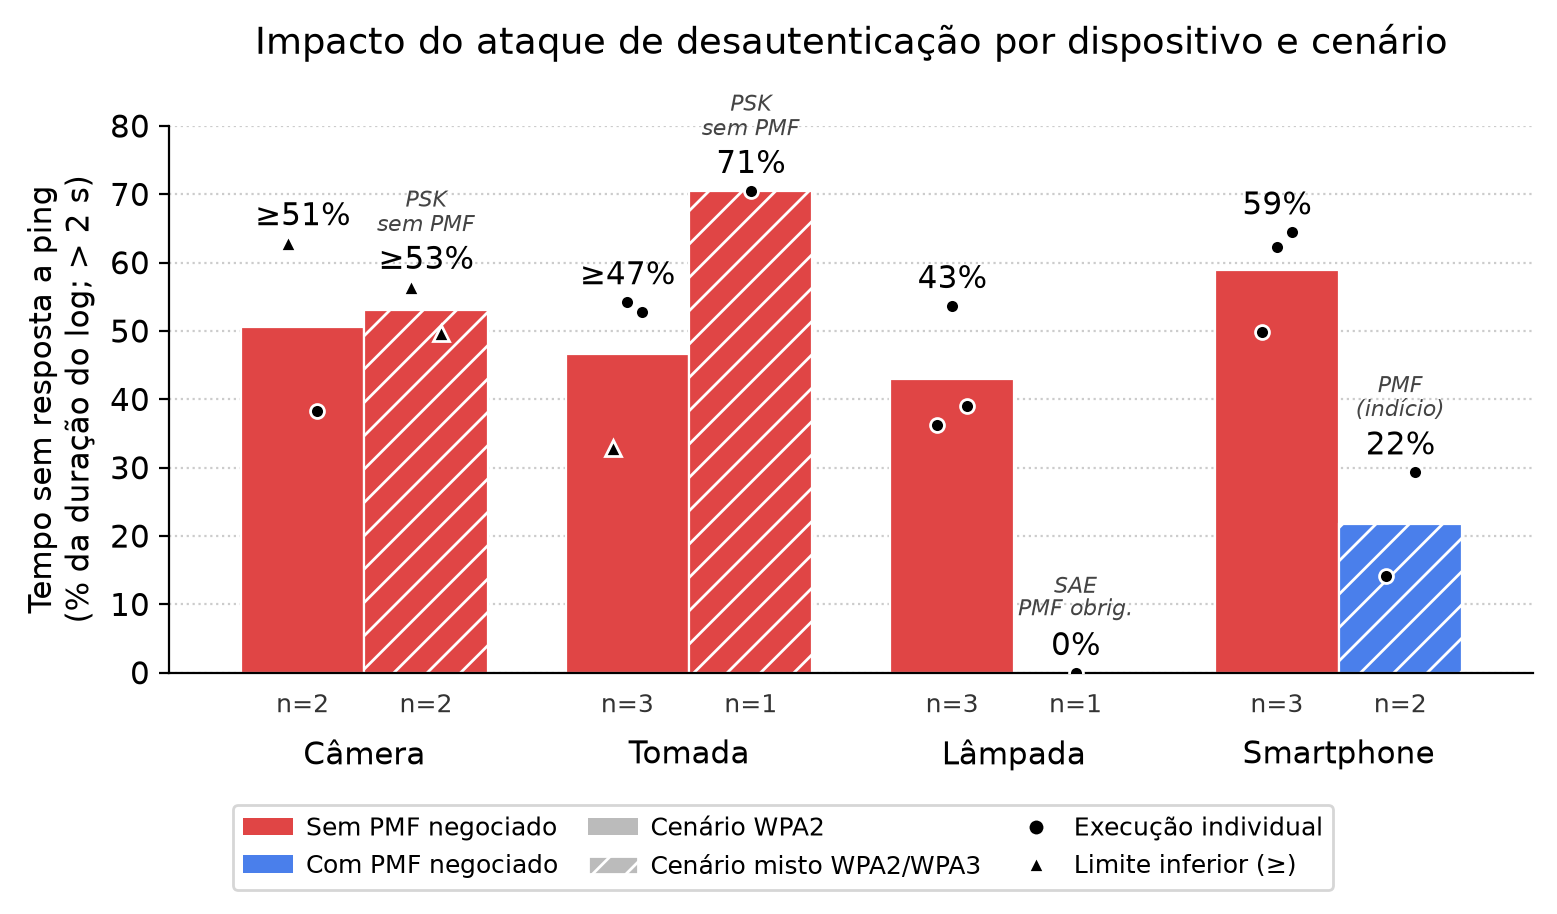
\includegraphics[width=0.95\textwidth]{comparacao_pmf.png}
\legend{Fonte: elaborado pelo autor a partir dos \textit{logs} de \textit{ping} dos ensaios (2026). Eixo vertical: tempo acumulado sem resposta ($>$2~s), excluídas as respostas duplicadas (\textit{DUP!}), dividido pela duração do \textit{log} de \textit{ping}; não equivale à perda de pacotes ICMP. Os pontos indicam as execuções individuais e $n$, o seu número; os triângulos marcam execuções cuja queda durou até o fim da captura. Barras com $\geq$ incluem pelo menos uma execução cuja queda durou até o fim da captura; o valor é um limite inferior da média, e não uma média propriamente dita. No cenário WPA2, a câmera aparece com \texttt{CAM\_WPA2\_R03} e \texttt{CAM\_WPA2\_R04}; \texttt{CAM\_WPA2\_R05} e \texttt{CAM\_WPA2\_R06} (invalidadas) e \texttt{CAM\_WPA2\_R08} (medida pela captura, não por \textit{ping}) não entram. Valores calculados pelo \textit{script} \texttt{src/analisa\_ping.py} e figura gerada por \texttt{src/figura\_comparacao\_pmf.py}. As janelas de ataque de cada execução constam das Tabelas~\ref{tab:registro-execucoes} e~\ref{tab:registro-metricas}.}
\end{figure}

A Figura~\ref{fig:ping_lampada} mostra, para a lâmpada, as respostas a \textit{ping} ao longo de uma execução de cada cenário. No cenário WPA2, em que a lâmpada se associou com PSK e sem PMF, as respostas cessaram pouco depois do início do ataque e só voltaram após o seu término, em um único intervalo de 40,1~s sem resposta. No modo misto, em que a lâmpada negociou SAE com PMF obrigatório, as respostas continuaram durante todo o ataque, sem nenhum intervalo maior que 2~s, embora o tempo de resposta tenha oscilado mais durante a janela de ataque.

\begin{figure}[htb]
\centering
\caption{Respostas a \textit{ping} da lâmpada durante o ataque nos cenários WPA2 e modo misto WPA2/WPA3}
\label{fig:ping_lampada}
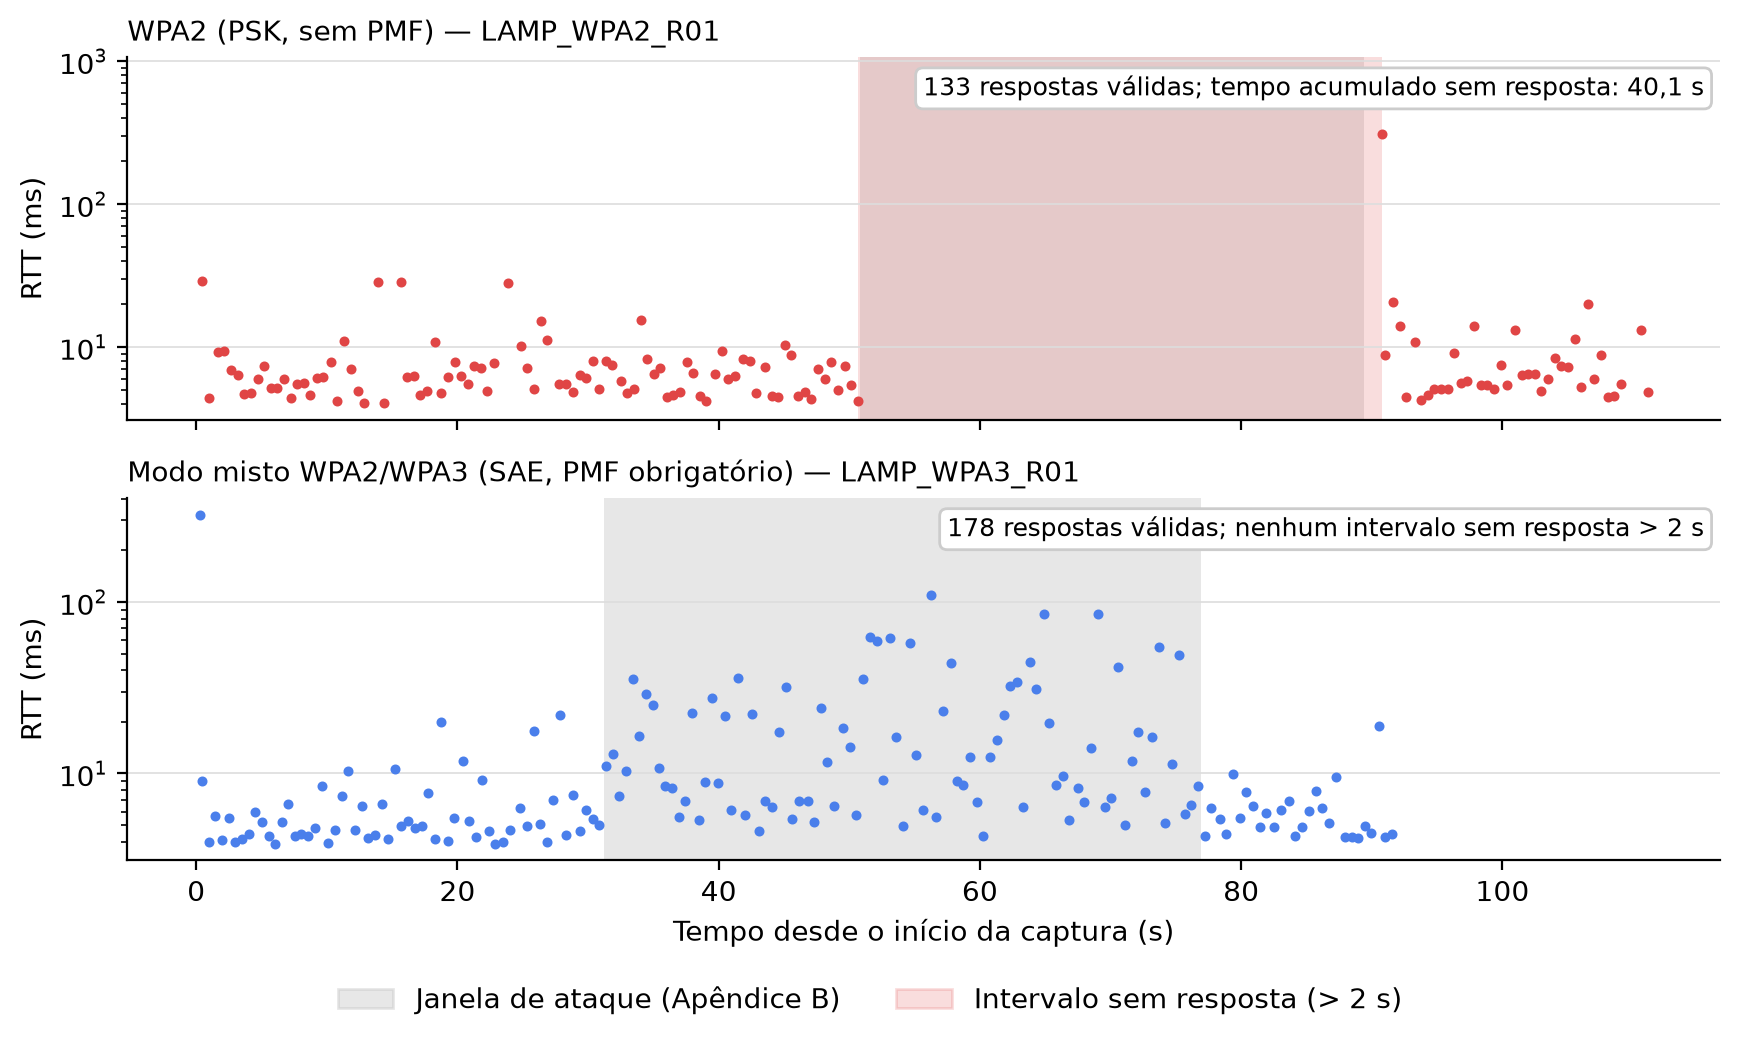
\includegraphics[width=0.95\textwidth]{ping_lampada.png}
\legend{Fonte: elaborado pelo autor a partir dos \textit{logs} de \textit{ping} das execuções \texttt{LAMP\_WPA2\_R01} e \texttt{LAMP\_WPA3\_R01} e do \textit{script} \texttt{src/figura\_ping\_lampada.py} (2026). Cada ponto é uma resposta válida (RTT em escala logarítmica). Faixa cinza: janela de ataque (Apêndice~\ref{sec:registro-execucoes}). Faixa vermelha: intervalo sem resposta maior que 2~s.}
\end{figure}

\subsection{Padrões de comportamento observados}
\label{subsec:padroes}

Os ensaios revelaram três padrões distintos de resposta ao ataque de desautenticação, todos no cenário WPA2 (sem PMF). A \textbf{câmera} interrompeu completamente o fluxo de vídeo. Em \texttt{CAM\_WPA2\_R03} não houve reassociação registrada na captura; em \texttt{CAM\_WPA2\_R04}, ela reassociou-se oito vezes durante o ataque, sempre seguida de nova desautenticação, e não se reassociou após o seu término. Em ambas, a função só foi restabelecida após reinício manual. A \textbf{tomada} e a \textbf{lâmpada} apresentaram um padrão intermitente na camada de enlace: eram desassociadas e reassociavam-se repetidamente durante o ataque (captura), sem voltar a responder ao \textit{ping} de forma estável até o seu término, com recuperação automática depois dele (exceto em \texttt{TOMADA\_WPA2\_R01}, cuja captura terminou antes da retomada). O \textbf{smartphone}, por sua vez, perdeu a conexão e não a restabeleceu sozinho, exibindo uma falsa mensagem de ``senha incorreta'' e só reconectando após intervenção manual do usuário na seleção da rede. Essa diversidade evidencia que o impacto de um mesmo ataque depende não apenas da camada de enlace, mas também da implementação de reconexão de cada dispositivo.

No cenário com WPA3 habilitado em modo misto, observou-se que a segurança é negociada por dispositivo, e não pela rede como um todo. A lâmpada, que negociou SAE com PMF obrigatório, manteve fluxo de dados contínuo e \textit{ping} sem intervalos sem resposta, apesar de 425 quadros de desautenticação a ela direcionados; o \textit{smartphone}, com indício indireto de PMF, manteve a associação mesmo sob mais de 500 quadros por execução nas execuções com ataque ao alvo, embora com intervalos sem resposta a \textit{ping}. Em contraste, a câmera e a tomada, que selecionaram PSK sem declarar suporte a PMF, apresentaram perda de associação e tempos sem resposta da mesma ordem do cenário WPA2; a câmera, como no cenário WPA2, não voltou a responder sem reinício manual, feito nas duas execuções. Esse padrão é compatível com a proteção esperada dos quadros de gerenciamento e indica que habilitar o WPA3 em modo misto não altera a exposição dos dispositivos IoT legados ao ataque de desautenticação.

\section{Discussão dos resultados}
\label{sec:discussao}

\subsection{Comparação entre o esperado e o obtido}

O referencial teórico discute a desautenticação como um mecanismo relacionado ao estado de autenticação e associação de estações, bem como os riscos de quadros de gerenciamento falsificados quando não há proteção apropriada. A identificação desse tipo de quadro no ensaio é coerente com o mecanismo investigado, porém não demonstra, por si só, quebra da criptografia de dados ou comprometimento de credenciais \cite{KohliosHayajneh2018}.



A comparação com o estudo de \citeonline{KristiyantoErnastuti2020}, já apresentado no referencial, deve preservar a diferença entre semelhança do arranjo experimental e equivalência de resultados. Ambos os recortes envolvem câmera IP, ponto de acesso e microcontrolador como instrumento de teste, e ambos confirmam a eficácia do ataque de desautenticação contra dispositivos IoT. Entretanto, os valores absolutos de indisponibilidade não são diretamente comparáveis, pois dependem do \textit{firmware}, da distância e da intensidade do ataque; a contribuição adicional deste trabalho está no registro, por dispositivo, da segurança efetivamente negociada (AKM e PMF) ao lado do impacto do ataque. Essa comparação não isola o efeito de um único fator: entre os dispositivos que mantiveram a associação e os que a perderam variaram, em conjunto, o AKM (SAE ou PSK), o PMF, o fabricante, o \textit{firmware} e a lógica de reconexão de cada equipamento. O resultado é, portanto, um padrão compatível com a proteção esperada dos quadros de gerenciamento pelo PMF, e não uma demonstração de causalidade exclusiva.



Em relação ao esperado, os objetivos específicos 1 e 2 foram atendidos, e os objetivos 3 e 4, parcialmente, conforme detalhado na Seção~\ref{sec:atendimento_objetivos}. O ambiente de ataque foi configurado e validado; os testes de desautenticação foram executados contra os quatro dispositivos; os tempos de indisponibilidade foram mensurados por \textit{ping} sincronizado, com três repetições para a tomada, a lâmpada e o \textit{smartphone} no cenário WPA2; e os dados de tráfego foram coletados e analisados para validar a eficácia técnica dos testes. A comparação entre os mecanismos de proteção foi realizada e mostrou que o rótulo configurado no roteador (WPA2 ou modo misto) não descreve, por si só, a situação de cada dispositivo: os dispositivos que operaram sem PMF apresentaram perda de conectividade em todos os ensaios --- com desassociação confirmada por novos quadros de autenticação e associação na maioria deles, exceto nas execuções \texttt{CAM\_WPA2\_R02} e \texttt{CAM\_WPA2\_R03}, em que a câmera não se reassociou e a desassociação não pôde ser confirmada pela captura ---, ao passo que a lâmpada, com SAE e PMF obrigatório, e o \textit{smartphone}, com indício indireto de PMF, mantiveram a associação. Esse padrão é compatível com a proteção esperada dos quadros de gerenciamento, mas, como SAE, PMF e o próprio dispositivo variaram juntos e não houve condição de WPA2 com PMF, não permite atribuir o resultado exclusivamente ao PMF.

O \textit{smartphone}, embora tenha mantido a associação no cenário misto, registrou em média $\approx$22\% do tempo sem resposta a \textit{ping} (14\% e 29\% em duas execuções). Uma hipótese para essa perda residual é a ocupação do canal pela emissão contínua de quadros de desautenticação, que compete pelo meio com o tráfego do dispositivo; outras explicações possíveis são a economia de energia do sistema operacional do \textit{smartphone} e perdas de recepção. Essas hipóteses não foram testadas neste trabalho, pois não se mediu a ocupação do canal nem se repetiu o ensaio sem o ataque nas mesmas condições.



A contribuição deste estudo consiste em demonstrar, de forma prática e mensurada, que uma plataforma de baixo custo (LILYGO T-Embed CC1101 Plus com \textit{firmware} Bruce) é capaz de desconectar dispositivos IoT comerciais por meio de ataques de desautenticação em redes IEEE 802.11 sem PMF, e em registrar que apenas os dispositivos que negociaram PMF mantiveram a associação, padrão compatível com a proteção esperada dos quadros de gerenciamento. Não se reivindica generalização para todos os roteadores, dispositivos ou \textit{firmwares} existentes, dado o caráter de estudo de caso com amostra intencional.

\subsection{Cenário crítico de aplicação: monitoramento de câmaras de vacinas}
\label{subsec:cenario_vacinas}

Esta subseção não relata um ensaio. Nenhum equipamento de monitoramento de vacinas foi testado na bancada: trata-se de uma análise de impacto que transporta os resultados medidos neste trabalho para um contexto em que a perda de disponibilidade da rede teria consequências maiores do que nos dispositivos residenciais avaliados. As fontes sobre monitoramento de vacinas citadas a seguir não tratam de ataques à rede sem fio; a ligação entre esse contexto e o ataque de desautenticação é uma inferência deste trabalho, apoiada nos resultados da bancada e no referencial sobre o IEEE~802.11.

Na Rede de Frio do Programa Nacional de Imunizações (PNI), as câmaras científicas refrigeradas usadas na conservação de imunobiológicos são projetadas para armazená-los entre 2~\textdegree{}C e 8~\textdegree{}C (BRASIL, \citeyear{BrasilRedeFrio2025}, p.~61). Para acompanhar essa faixa, a literatura descreve sistemas de monitoramento baseados em microcontroladores com Wi-Fi, que enviam as leituras de temperatura a serviços em nuvem e emitem alertas remotos. \citeonline{Harrabi2024} empregaram um ESP32, da mesma família de SoCs da Espressif que o ESP32-S3 usado como plataforma de ataque neste trabalho, para monitorar a temperatura de refrigeradores de vacinas, transmitir os dados sem fio e enviar alertas a um aplicativo de celular em situações como falha do sensor, queda de energia e porta aberta. \citeonline{PoochayaWidjaja2018} descrevem um sistema baseado em Wi-Fi e IoT que avisa o farmacêutico quando o refrigerador sai da faixa de temperatura, e \citeonline{Adilah2025} combinam um ESP32 com armazenamento em nuvem, registro em cartão de memória local e alertas por aplicativo de mensagens, avaliados em uma câmara fria real. No contexto brasileiro, \citeonline{Barbosa2022} relata casos de doses descartadas por oscilação de temperatura e propõe um dispositivo IoT para monitorar a temperatura das vacinas em campanhas de vacinação extramuros, e \citeonline{SilvaSantos2023} desenvolveram uma aplicação de monitoramento em tempo real, com registro histórico e alertas de temperatura, voltada à Rede de Frio do PNI.

Nesses sistemas, convém separar a função local, de refrigeração, da função de rede, de telemetria e alarme remoto. O ataque de desautenticação atua sobre a segunda: afeta a disponibilidade da comunicação entre o sensor e o ponto de acesso \cite{KohliosHayajneh2018}, mas não desliga o compressor nem altera a temperatura interna. Durante o ataque, a refrigeração continuaria funcionando; o que se perderia seriam o envio das leituras e o alarme remoto.

Os resultados medidos indicam como essa perda poderia ocorrer. Nas condições estudadas, os dispositivos associados sem PMF perderam a conectividade enquanto o ataque estava ativo (Figura~\ref{fig:comparacao_pmf}). No cenário WPA2, a tomada ficou sem responder a \textit{ping} por $\geq$45,4~s, 106,4~s e 93,6~s (o primeiro valor é limite inferior), e a lâmpada, por 40,1~s a 52,8~s ($n=3$ cada); ambas se reassociaram repetidamente durante o ataque e voltaram a responder de forma automática depois do seu término, exceto em uma execução da tomada, cuja captura terminou antes da retomada (Seção~\ref{subsec:padroes}). A câmera teve o comportamento mais grave para um cenário de monitoramento: não recuperou a conectividade sozinha em nenhuma das quatro execuções medidas por \textit{ping} e precisou de reinício manual em todas (duas em WPA2 e duas no modo misto), assim como no ensaio piloto. Em três dessas execuções, a queda durou até o fim da captura e foi registrada apenas como limite inferior, de pelo menos 160~s na mais longa (Tabelas~\ref{tab:consolidacao-resultados} e~\ref{tab:consolidacao-recuperacao}). Um registrador de temperatura que reagisse como a câmera ficaria sem enviar leituras e sem alarme remoto até que alguém percebesse a falha e reiniciasse o equipamento.

O ataque não tem duração máxima: na plataforma utilizada, a emissão dos quadros de desautenticação continua até que o ataque seja desativado no menu do Bruce ou que a placa seja desligada. Nos ensaios, cada janela de ataque foi encerrada manualmente pelo pesquisador e durou entre cerca de 18~s (ensaio piloto) e 120~s (Tabela~\ref{tab:registro-execucoes}). Assim, enquanto a placa permanecesse ligada e ao alcance do ponto de acesso, o atacante poderia manter a interrupção pelo tempo que quisesse. O que não foi testado é o efeito de um ataque prolongado, por horas, sobre os dispositivos, nem a autonomia da bateria da plataforma nessa condição.

Em contraste, a lâmpada, que negociou SAE com PMF obrigatório no modo misto, não apresentou intervalo sem resposta a \textit{ping}, apesar de 425 quadros de desautenticação a ela direcionados ($n=1$), e o \textit{smartphone}, com indício indireto de PMF, manteve a associação ($n=2$), embora com 22,8~s e 24,7~s sem resposta, o que é coerente com o fato de o PMF proteger os quadros de gerenciamento sem garantir a disponibilidade completa do canal \cite{CiscoMFP2024}. O modo misto mostra ainda o limite de proteger apenas o roteador: com o ponto de acesso oferecendo PMF, a câmera e a tomada associaram-se sem ele e voltaram a perder a conectividade (Tabela~\ref{tab:negociacao-seguranca}). Em um serviço de saúde, habilitar o WPA3 no roteador em modo misto não protegeria um sensor legado que se associasse com WPA2 sem PMF.

A interrupção da telemetria, isoladamente, não comprometeria as vacinas, pois a temperatura continuaria controlada pelo equipamento. O risco estaria na coincidência entre a interrupção e uma falha real, como queda de energia, porta mal fechada ou defeito no compressor, enquanto o alarme remoto estivesse mudo. Sem o alarme, a equipe poderia não agir a tempo, e o lote poderia ser perdido, com possível atraso da vacinação e custo para o serviço de saúde. Este trabalho não estima a probabilidade dessa coincidência nem o valor das perdas.

Com base nos resultados e nas fontes citadas, sugerem-se as seguintes medidas de mitigação para esse tipo de aplicação:

\begin{itemize}
    \item sensor e ponto de acesso que negociem PMF, de preferência com WPA3 ou com WPA2 e PMF obrigatório, verificando a segurança efetivamente negociada na associação, e não apenas a configuração do roteador (Apêndice~\ref{sec:evidencias-rsn});
    \item alarme local, sonoro e visual, no próprio equipamento, independente da rede;
    \item registrador com memória local, para que o histórico de temperatura não se perca durante a interrupção, como o registrador eletrônico (\textit{datalogger}) que o manual da Rede de Frio recomenda manter nas câmaras frias, em paralelo ao registrador do equipamento e ininterruptamente (BRASIL, \citeyear{BrasilRedeFrio2025}, p.~68), ou o cartão de memória empregado por \citeonline{Adilah2025};
    \item alerta por ausência de dados na plataforma de monitoramento, que trate a falta de leituras por um intervalo definido pelo serviço como condição de alarme;
    \item canal alternativo para o alarme crítico, como a rede celular ou LoRa (\textit{Long Range}), que não dependa do Wi-Fi.
\end{itemize}

Essa análise tem limites explícitos. Nenhum registrador de temperatura de vacinas foi testado, e a análise supõe um sensor com comportamento semelhante ao dos dispositivos IoT sem PMF da bancada. O comportamento real dependeria do \textit{firmware} de cada equipamento, em especial da lógica de reconexão e da existência de memória e de alarme locais, e poderia ser melhor ou pior do que o observado. Os números citados nesta subseção são os medidos na bancada, com os respectivos $n$, e não estimativas para equipamentos de saúde.

\subsection{Limitações}
\label{subsec:limitacoes_resultados}

As principais limitações são: o número reduzido de execuções da câmera medidas por \textit{ping} no cenário WPA2 (duas, \texttt{CAM\_WPA2\_R03} e \texttt{CAM\_WPA2\_R04}), sendo que, na primeira, o intervalo sem resposta tem apenas limite inferior, pois a conectividade não voltou antes do encerramento da captura, o que também ocorreu nas duas execuções da câmera no modo misto (\texttt{CAM\_WPA2\_R02} e \texttt{CAM\_WPA3\_R01}) e na \texttt{TOMADA\_WPA2\_R01}, cujos intervalos sem resposta são igualmente limites inferiores; o número reduzido de repetições no cenário em modo misto (uma execução para a tomada e para a lâmpada, duas para a câmera e para o \textit{smartphone}); e a impossibilidade de avaliar os dispositivos IoT em WPA3 puro, já que câmera e tomada não suportam esse protocolo e não se associam a uma rede exclusivamente WPA3. Também não houve condição de WPA2 com PMF: no cenário WPA2 o ponto de acesso não ofereceu PMF, e no cenário misto câmera e tomada não declararam suporte a ele. Por isso, SAE, PMF e o próprio dispositivo variaram em conjunto, e o efeito do PMF não pôde ser separado do efeito do AKM e da implementação de cada equipamento. Nos ensaios da tomada em WPA2, a captura registrou proporção de quadros de desautenticação em difusão muito maior que nos demais ensaios considerados na análise, com o mesmo método de ataque e causa não investigada; essa diferença limita a comparação direta desses ensaios com os demais (Seção~\ref{sec:condicoes_experimentais}). Quanto à evidência da segurança negociada, o AKM do \textit{smartphone} no cenário misto não foi observado, pois nenhuma associação dele foi capturada, e a associação da lâmpada com SAE foi registrada em captura dedicada, e não durante o ensaio de ataque (Apêndice~\ref{sec:evidencias-rsn}). A captura por rádio está sujeita a condições de recepção e não constitui inventário integral de toda transmissão no canal. Além disso, o tempo de indisponibilidade foi medido por \textit{ping}, o que reflete a disponibilidade de rede, mas não necessariamente a recuperação completa da função da aplicação (por exemplo, o fluxo de vídeo da câmera). Por fim, a plataforma de ataque e a estação de captura operam apenas em 2,4~GHz, de modo que dispositivos exclusivamente em 5~GHz não puderam ser avaliados diretamente, conforme discutido na Seção~\ref{subsec:consolidacao_resultados}. O cenário de monitoramento de câmaras de vacinas (Seção~\ref{subsec:cenario_vacinas}) é analítico, e não experimental: nenhum registrador de temperatura foi testado, e a transposição dos resultados supõe um sensor com comportamento semelhante ao dos dispositivos sem PMF da bancada.



O uso do aplicativo e da internet também introduz dependências que devem ser diferenciadas da associação Wi-Fi. Ausência de imagem não comprova isoladamente perda da conexão de rádio; da mesma forma, presença de quadros de dados não demonstra atualização correta do vídeo. A retomada da associação e a retomada da função devem ser registradas como eventos distintos.

\subsection{Pontos fortes}

Entre os pontos fortes do estudo estão a separação entre a plataforma de intervenção e o instrumento de captura, a identificação dos alvos por cruzamento com o painel do roteador e com os endereços dos quadros, a medição sincronizada da indisponibilidade por \textit{ping}, a realização de três repetições para a tomada, a lâmpada e o \textit{smartphone} no cenário WPA2 e a verificação, a partir do elemento RSN dos quadros de associação, da segurança negociada por cada dispositivo. Esse último ponto permitiu distinguir a configuração do roteador da segurança efetivamente negociada e relacionar a manutenção da associação à presença do PMF, ainda que sem isolá-lo dos demais fatores.

\section{Síntese dos resultados}
\label{sec:sintese_resultados}

Em síntese, no cenário WPA2, em que o ponto de acesso não ofereceu PMF, a tomada, a lâmpada e o \textit{smartphone} apresentaram intervalos sem resposta a \textit{ping} durante os ensaios, correspondentes a $\approx$43\% a $\approx$59\% da duração dos \textit{logs}, sendo o valor da tomada ($\geq$47\%) um limite inferior (Figura~\ref{fig:comparacao_pmf}), com padrões de recuperação distintos: reconexão automática intermitente na tomada e na lâmpada e reconexão manual no \textit{smartphone}; a câmera, nesse cenário, teve duas execuções com \textit{ping} (\texttt{CAM\_WPA2\_R03} e \texttt{CAM\_WPA2\_R04}), em que a conectividade só retornou após reinício manual. No modo misto, câmera e tomada negociaram PSK sem PMF e voltaram a apresentar perda de conectividade, e a câmera novamente só foi restabelecida por reinício manual; a lâmpada, com SAE e PMF obrigatório, não apresentou intervalos sem resposta; e o \textit{smartphone}, com indício indireto de PMF, manteve a associação, mas registrou em média $\approx$22\% do tempo sem resposta. A resposta ao problema de pesquisa, as contribuições e as limitações do estudo são tratadas no Capítulo~\ref{cap:conclusao}.
